\chapter{Introduction}\label{chap:introduction}

A neural network, also known as an Artificial Neural Network (ANN), is an algorithm that mimics the way a human brain operates. It took millions of years of evolution for the human brain to achieve the level of intelligence we observe today. This intelligence helps us quickly interpret and evaluate what we see in our surroundings. For example, consider the following image of hand-written digits from the MNIST dataset \cite{mnist}:

\begin{figure}[h]
	\centering
	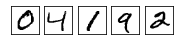
\includegraphics[width=0.5\linewidth]{images/introduction/digits.png}
	\caption[Hand-written digits]%
	{\textbf{Hand-written digits}: Each hand-written digit is a $28\times28$ pixel grayscale image. The entire MNIST dataset contains a total of $70000$ such images that split into a training set of $60000$ images and a test set of $10000$ images.}
	\label{fig:digits}
\end{figure}

One can quickly recognize these digits as $04192$, thanks to the network of billions of neurons available in our brain that makes it easy to identify visual patterns. Past experiences and memories stored in our brain make this process so simple that it happens subconsciously most of the time. This simple process becomes much more difficult when we try to write computer programs to identify similar patterns due to the lack of precise rules and hundreds of exceptions and varieties of a single pattern.

Neural networks tackle this problem by inferring rules from a large set of related training data. For example, to train a neural network to efficiently recognize hand-written digits shown in figure \ref{fig:digits}, a dataset large enough to include different styles of hand-written digits is needed.

Neural networks and their variations such as Convolutional Neural Networks (CNNs), Recurrent Neural Networks (RNNs) are proven to be useful in many different application areas such as image recognition \cite{image_recon}, machine translation \cite{russian}, recommender systems \cite{recommender}. Despite this state-of-the-art performance, neural networks are computationally complex and memory-intensive due to their deep structures.

Sparse Neural Networks are a viable option to make neural networks less complex and make them memory efficient. Such sparsity in neural networks can be induced by pruning weights, utilizing skip connections, or generating random architectures based on graphs. Sparsity in a neural network can reduce that network's size by many times with little to no drop in performance \cite{sparse_nn, dey, liu}. Therefore, in this thesis, we implement two different ways to achieve sparsity in Recurrent Neural Networks and analyze its performance impact.


% -----------------------------------------------------------------------------------------------------------
% ------------------------------------------------ MOTIVATION -----------------------------------------------
% -----------------------------------------------------------------------------------------------------------

\section{Motivation}\label{section:motivation}

As stated before, deep neural networks are likely to have an increased performance but at the cost of higher complexity and increased fast memory requirements. One way to mitigate this issue while maintaining the performance is to introduce sparsity into a network's connections \cite{deep_res}. For example, Mao et al. in \cite{mao} report a higher-compression ratio with coarse-grained pruning without loss of accuracy while saving about twice the memory references. Similarly, Sun et al. in \cite{sparse_face} reported that the sparse ConvNet model, which only has 12\% of the original parameters, still performs similarly to the baseline model.

These are just a few examples where Sparse Neural Networks have proven advantageous in time, energy, and memory savings. Sparsity in traditional neural networks and CNNs is studied widely by many researchers but is not explored much in Recurrent Neural Networks that are difficult to train due to their nonlinear iterative nature. Sparse structures in traditional neural networks have shown a promise of training potential \cite{sparse_nn} which, if applied to Recurrent Neural Networks, can also make training RNNs less difficult by reducing their network size while retaining their performance.

% -----------------------------------------------------------------------------------------------------------
% -------------------------------------------- RESEARCH QUESTIONS -------------------------------------------
% -----------------------------------------------------------------------------------------------------------

\newpage
\section{Research questions}\label{section:research_questions}

The primary research goal of this master thesis is to investigate the effects of sparse structure on the performance of the Recurrent Neural Networks and its variants, namely Long Short-Term Memory and Gated Recurrent Unit. To do so, we have defined the following set of correlated research questions:

\begin{enumerate}
	\item\label{rq:q1} What is the effect of weights pruning on a recurrent network's accuracy?
	    
	\item\label{rq:q2} What percentage of weights pruning is permissible without triggering a significant reduction in the performance?
	    
	\item\label{rq:q3} After pruning a certain percent of weights, if we see a significant reduction in the accuracy,  how many re-training epochs can regain accuracy?
	    
	\item\label{rq:q4} How does a randomly structured recurrent network's performance correlate with the graph properties of its internal structure?
	
	\item\label{rq:q5} Is it possible to predict a randomly structured recurrent network's performance using the graph properties of its base random graph?
\end{enumerate}

We will answer all these questions for four different recurrent networks, namely RNN with Tanh nonlinearity (RNN-Tanh), RNN with ReLU nonlinearity (RNN-ReLU), Long Short-Term Memory (LSTM), and Gated Recurrent Unit (GRU), by following the approach explained in section \ref{section:proposed_approach}.

% -----------------------------------------------------------------------------------------------------------
% -------------------------------------------- PROPOSED APPROACH --------------------------------------------
% -----------------------------------------------------------------------------------------------------------

\newpage
\section{Proposed approach}\label{section:proposed_approach}

To investigate the effects of sparse structures in recurrent networks, we propose the following three experiments:
\begin{enumerate}
	\item \textbf{Investigating the effects of weights pruning on recurrent networks}: \\
	    In this experiment, we prune input-to-hidden and hidden-to-hidden weights, both simultaneously and individually.
	    
	    We start by training a recurrent network on a dataset for a certain number of epochs. Once this training is complete, we follow the process shown in the following flowchart:
	    
	    \begin{figure}[h]
            \centering
            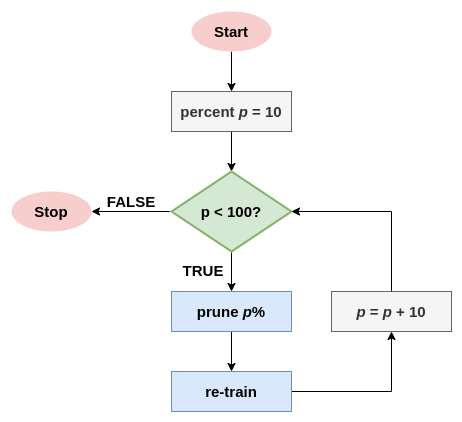
\includegraphics[width=0.5\linewidth]{images/introduction/flow_1.png}
            \caption[Flowchart for the pruning experiment]{The basic flowchart depicting the process of pruning and re-training a trained recurrent network.}
            \label{fig:flowchart_pruning}
        \end{figure}
        
    	 To outline this flowchart, once the initial training is complete, retrieve the learned weights of the trained model, prune the lower $p\%$ of weights (where $p \in \mathbb{Z}:p \in [1, 100]$), and re-train this pruned model to check for the number of epochs required to regain accuracy.
    	 
    	 This experiment will help answer research questions \ref{rq:q1}, \ref{rq:q2}, and \ref{rq:q3}.
    	
	\item \textbf{Analyzing the performance of recurrent networks with randomly structured recurrent networks}: \\
	    We start by generating randomly structured neural networks by following the technique described by Stier et al. in \cite{julian} that generate Sparse Neural Networks.

        After generating Sparse Neural Networks, we introduce recurrent connections to generate Sparse RNNs. These recurrent connections are necessary to make each subsequent run dependent on the previous run.

        Once we have Sparse RNNs, we train them on a dataset and compute the correlation between its accuracy and its internal structure's graph properties.
        
        This experiment will help answer the \ref{rq:q4}th research question.
	    
    \item \textbf{Performance prediction of a randomly structured neural network:}: \\
        Once we have trained Sparse RNNs, we train three different regressor algorithms with graph properties as features and corresponding accuracy as the target. Since this is a regression problem, we finally report an R-squared value for each RNN variant and each regressor algorithm.
        
        This experiment will help answer the \ref{rq:q5}th research question.
\end{enumerate}

All these three approaches are described in detail in the later chapters.

% -----------------------------------------------------------------------------------------------------------
% ------------------------------------------------ STRUCTURE ------------------------------------------------
% -----------------------------------------------------------------------------------------------------------